\documentclass{beamer}
\usepackage[utf8]{inputenc}
\usepackage{graphicx}
\author[Sowmya Vajjala]{Instructor: Sowmya Vajjala}


\title[LING 120]{LING 120, Fall 2017: \\ Language and Computers}
%\subtitle{based on Chapter 10 of the textbook}

\date{15 Sep 2017}

\institute{Iowa State University, USA}

%%%%%%%%%%%%%%%%%%%%%%%%%%%

\begin{document}

\begin{frame}\titlepage
\end{frame}

\begin{frame}
\frametitle{Class outline}%5minutes
\begin{enumerate}
\item Discussion on question from last class
\item Mobile apps and language learning %10min
\item View - a system for practicing grammar %5min
\item LTS to teach writing %Link 5min
\item LTS to teach speaking 
\item LTS to teach listening %Link.  5min
\item Specialized LTS %RWT 
\item Language Tutoring Systems - conclusion  %5 min 
%remaining time: exercise. - may be on how to evaluate short answer questions?
\end{enumerate}
\end{frame}

\begin{frame} %15min?
\frametitle{Attendance exercise for last class} 
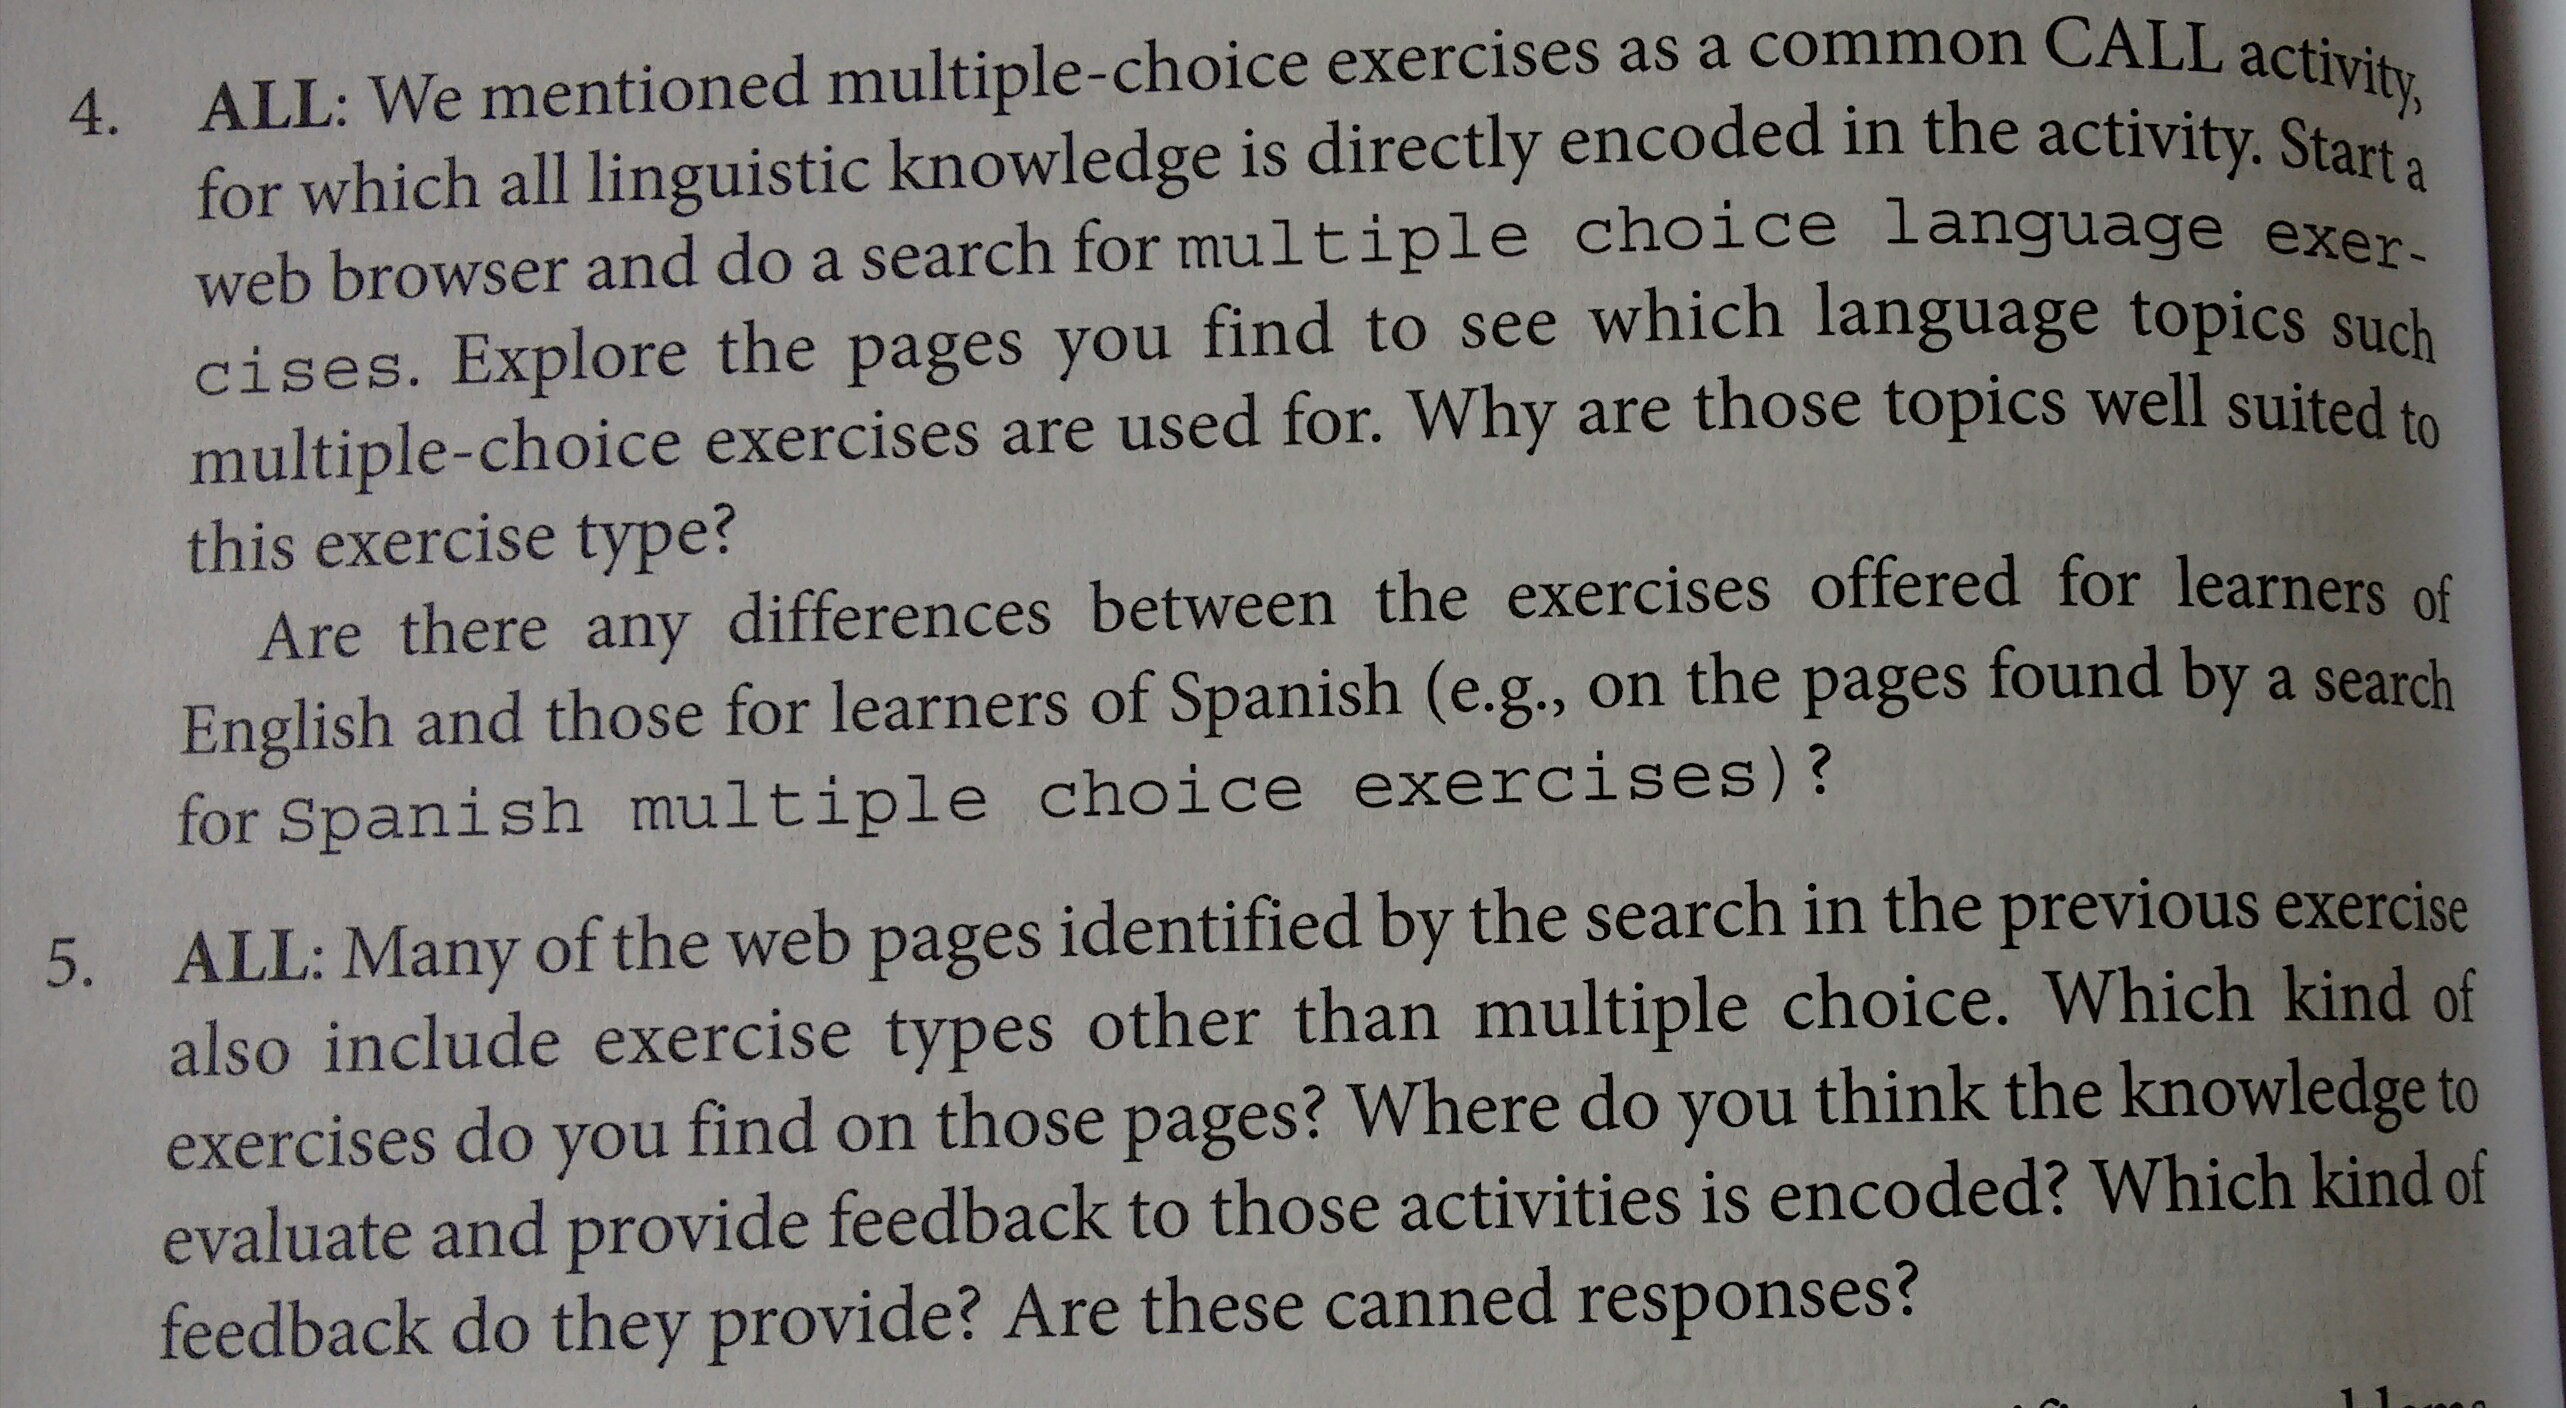
\includegraphics[width=0.99\textwidth]{13SepExercise.jpg}
\end{frame}

\begin{frame}
\frametitle{Main points from your Responses}
\begin{itemize}
\item Multiple choice questions about tense make sense because knowing the word is not sufficient for getting the right tense.
\item In Spanish, there were questions focusing on noun-gender, verb conjugation which may not make sense in English. 
\item One student reported on Arabic exercises (!), focusing on word order. 
\item Feedback given by the system depended on how unsure the learner was (chosen by button click) in one case. 
\item Feedback is canned in many other cases. 
\item Most multiple choice questions seem grammar based, not vocabulary based. 
\end{itemize}
\end{frame}

\begin{frame}
\frametitle{Mobile Apps and Language Learning}
\begin{itemize}
\item Apps with structured courses (Duolingo, Babbel - web interface available)
\item Apps with flashcards etc to remember words (Memrise)
\item Educational games (MindSnacks)
\item Practicing communication (HelloTalk)
\item Pronunciation training (ElsaSpeak)
\end{itemize}
more: \url{https://www.lingualift.com/blog/best-language-learning-apps/}
\\ note: some of them are frame based. Some of them use language processing, machine learning, speech recognition and other technologies.
\end{frame}%5min

\begin{frame}
\frametitle{Not tutoring, but letting you practice with real texts}
VIEW: \url{http://sifnos.sfs.uni-tuebingen.de/VIEW/} - quick demo
\end{frame} %10 min

\begin{frame}
\frametitle{LTS that give feedback on writing: }
\begin{itemize}
\item CyWrite@ISU: \url{https://cywrite.engl.iastate.edu/wp/}
\item eRater by ETS: \url{https://www.ets.org/criterion/} \\ (demo: \url{https://vimeo.com/30553836})
\item WriteToLearn: \url{http://www.//writetolearn.net} \\ (demo: \url{https://goo.gl/vEV3o7})
\item general purpose writing feedback: Grammarly.com 
\end{itemize}
... and so on. 
\end{frame} %10-15min

\begin{frame}
\frametitle{Teaching to Speak and Listen}
\begin{itemize}
\item GoldenSpeaker@ISU: \url{http://goldenspeaker.las.iastate.edu}
\item Project Listen @CMU: \url{http://www.cs.cmu.edu/\~./listen/}
\item 2 demo videos of Project Listen
\end{itemize}
\end{frame} %10-15 min

\begin{frame}
\frametitle{Teaching to Speak and Listen}
Specialized writing tutor: Research Writing Tutor@ISU \\ 
\url{https://vimeo.com/90669213}
\end{frame}

\begin{frame}
\frametitle{CALL/LTS: Conclusion}
\begin{itemize}
\item Interesting mix of computer science, linguistics, psychology, human-computer interaction studies, language teaching etc.
\item Existing software range from neatly made interfaces that are not "intelligent" to those that adapt to the learner through machine learning and NLP techniques.
\end{itemize}
\end{frame}

\begin{frame}
\frametitle{Next Week}
\begin{itemize}
\item Topic 4: Searching
\item Readings: Chapter 4
\item Assignment 2 is due next week
\item I will announce mid-term topics and teams next week. 
\end{itemize}
\end{frame}

\begin{frame}
\frametitle{Attendance Exercise}
Assume you are given the task of designing a software that can automatically score short answers from students about whatever they read (science, maths, any subject). 
How will you go about this? What kind of tasks should that system do? What are the features we should look at to evaluate student answers? \\
a) if we have a target answer \\
b) if we do not have a target answer
\\ \medskip (write your answers on a sheet of paper and return to me. You can also post on Canvas in the discussion forum for today's date)
\end{frame}


\end{document}
